% Chapter Template

\chapter{State-of-the-art} % Main chapter title

\label{Chapter2} % Change X to a consecutive number; for referencing this chapter elsewhere, use \ref{ChapterX}

\lhead{Chapter 2. \emph{State-of-the-art}} % Change X to a consecutive number; this is for the header on each page - perhaps a shortened title

%----------------------------------------------------------------------------------------
%	SECTION 1
%----------------------------------------------------------------------------------------
\section{Introduction}
This chapter will cover off research literature in the field of credit risk and predicting default of SME customers in Financial institutions. The first couple of sections will cover off the field of SME, detailing SME definitions, credit risk and how macro economic features are used to in SME and economic credit risk. It will discuss challenges in the past in the field such as lack of common definitions and common statistics that could be used to straighten the sector. The literature for macro-economic factors is reviewed and it is noted that there has not much time spent researching how macro-economic factors affect SME credit and credit risk as a whole. It finishes detailing how there has been success using macro-economic factors in Italy, Portugal in predicting credit risk utilising features based on default rate and unemployment by location or area.   

The chapter will also review research literature in the field of knowledge discovery, data mining and with a focus on predictive modelling. Knowledge discovery and data mining will be explained and illustrated with frameworks and methodologies about how to approach tasks in each. The literature is reviewed to understand the processes, prediction algorithms, feature selection methods,  validation methods and performance measures to understand how to build a predictive model to predict SME customers that are likely to default i.e. risky customers. One key observation in building a model to how predict what customers will default is that there tends to a very large class imbalance in the dataset e.g. there will be a much larger proportion of good/well behaving than bad/poorly performing customers. There are many ways of addressing this class imbalance by either manipulating the data set through sampling techniques or through fine tuning the algorithm by alternating input parameters tailored to the imbalance in the dataset.

\section{SME Definition}
The most common definition for an SME is a registered business that with less than 250 employees \citep{ifc_sme_2009}, however this definition is not always consistent and can vary from country to country, financial institution to financial institution. 

At a European level an SME, business is categorised as SME if they have two hundred and fifty people or less employed and if the annual turnover not surpassing 50 million euro , and/or an annual balance sheet not surpassing 43 million euro\footnote{\url{http://isme.ie/advice/sme-facts-faq}}\footnote{\url{https://www.enterprise-ireland.com/en/About-Us/Our-Clients/SME-Definition.html}}.cSMEs can also be broken down further into smaller subcategories, micro enterprises are defined as businesses that employ fewer than ten people, have annual turnover below 2 million and annual balance sheet total not surpassing 2 million. Small enterprises are defined as businesses that have employed between ten and fifty people, have annual turnover below 10 million and annual balance sheet total below 10 million. Medium enterprises are defined as businesses that have employed between fifty and two hundred and fifty people employed have an annual turnover less than 50 million and an annual balance sheet total below 43 million.\footnote{\url{http://www.cgap.org/financialindicators}}

Worldwide the most common method by regulators for defining businesses as SME are based the number of people they have employed, sales/turnover or/and loan size \cite{ardic_small_2011}.

In 2004 at an OECD conference on SMEs there were two key recommendations made economies of member and non-member states\footnote{Second OECD Conference of Ministers Responsible for Small and Medium-Sized Enterprises (SMEs), Istanbul,2004. \url{http://www.oecd.org/cfe/smes/31919278.pdf}}: (i) develop SME statistics that can be compared internationally, and (ii) establish a common definition and set rules for what an SME is. Without these statistics and definitions in place it would be more difficult to deploy programs that aim to expand and strengthen the SME sector\citep{ardic_small_2011}


\section{Credit Scoring Best Practice}
\textit{Hand, D. J. (2005). Good practice in retail credit score-card assessment. Journal of the
Operational Research Society, 56, 1109–1117.}
%----------------------------------------------------------------------------------------
%	SECTION 2
%----------------------------------------------------------------------------------------
\section{Importance and Methods of SME Credit Risk Assessment}
Recent research indicates that SME development is closely linked with economic growth, \cite{beck_smes_2005} research indicates there is strong correlations between the size of an economies SME sector and economic growth. After the recent global financial crisis of 2008 and 2009 it is important to note that the SME segment is recognised as one of the important factors to a sustainable employment and economic recovery \citep{lawless_smes_2012}. \cite{lawless_smes_2012} also note that this mainly due to the indigenous, employment-intensive nature of SMEs. SMEs are of major importance to many economies, in Ireland SME account for 68 percent of employment and 99 percent of firms in the private sector \cite{lawless_irish_2012}. Since the financially crisis SMEs have been hampered constraints on the ability to get credit due policies and regulations, however it has been recognised internationally that businesses that are credit constrained engage with less economically valuable and growth enhancing activity such as job and employment creation than similar unconstrained businesses \citep{campello_real_2010}. This means that financial institutions sit at the heart of the economy making decisions on what businesses to bet/gamble for one their own profits but also promote growth leading to a sustainable employment and economy. This requires financial institution credit models to be aware at all times of the current economic factors that are influencing good and bad credit decision. 

One of the fundamentals of building a prediction models on SME lending is to look at previous lending patterns and what is currently on the the financial institutions books \citep{lawless_irish_2012}. It is essential to test and evaluate the predictiveness of data from a wide variety of sources \citep{lawless_smes_2012}. This allows you to build a predictive model with as complete picture of the SME book as possible. To do this financial institutions deploy credit scoring to evaluate the credit risk of both existing and prospective \citep{kennedy_credit_2013}. Credit scoring is essentially the prediction models and methods that are deployed by lenders assess the credit risk of new or existing customers. These methods will attempt to put customers into a class of good or bad customer. Typically these scoring models are generally combine two approaches to score a customer, application scoring and behavioural scoring. The application model will assess applicant details which will be based mainly on their demographics. The behavioural model will assess the risk of the recent transactions of the existing customers. 

There two approaches to credit score modelling a widely used in the literature and adopted by \subjectname\ in industry but their evidence in the literature that supports macro economic model behaving could also be used. The success of macro economic factors will be discussed in the next section.

Data mining  is integral to credit scoring which will be discussed in Section \ref{sec:dataMining}, it applies many techniques and methods that are required for credit scoring.

%----------------------------------------------------------------------------------------
%	SECTION 3
%----------------------------------------------------------------------------------------
\section{Macro Area Features affecting SME and Economic Credit Risk}
\cite{hackbarth_capital_2006} note that even though there has been a substantial amount of time  understanding and developing the credit risk literature, there not been much time spent researching how macroeconomic factors affect credit risk.  \cite{hackbarth_capital_2006} finds this strange based on anecdotal suggestions from institutions that economic business cycle is an important feature when calculating the probability of default of a customer. One example of this is during a recession we know consumers are less likely to spend money on discretionary goods or luxuries thus as a result businesses in a sector that offer these goods credit risk will most likely rise. In their research they found that macroeconomic conditions do have an impact on credit risk.

\cite{fama_term_1986} notes how over the counter derivatives broker-dealers measure risk using individual counter-parties details but also geographic data and performance indicators of other industry groups. The \cite{derivatives_policy_group_framework_1995} \footnote{The Derivatives Policy Group was made up of representatives of CS First Boston, Goldman Sachs, Morgan Stanley, Merrill Lynch, Salomon Brothers, and Lehman Brothers} also made recommendations that credit exposure was measured by geography and industry exposure when calculating credit risk.

Banks can also suffer from a risk known as the \textit{winners curse}. In banking this is a scenario where other banks credit risk models score a customer too risky to lend to. That party then arrives at "our bank" where "our model" scores them as a good or likely to repay customer and decide to lend to them. As a result "our bank" will take on an excessive amount of risk that where other banks expected loses \citep{duffie_credit_2012}. \cite{duffie_credit_2012} also discuss how banks can mitigate their risk to the winners curse by including metrics such as borrowing rates and credit risk concentration limits by area or location.

Based on the Italian market, \citep{di_pietro_regional} investigated if SMEs experienced different levels of default rate based on their regional location. They investigated the business cycles of these areas and looked at identifying which macroeconomic features were the most influential in predicting default. In their experiment they divided Italy into five areas, centre, north-east, north-west, south, and the islands. They found in their analysis confirmed that there statistically a significant difference between default rates in the areas which can be seen in Fig. \ref{fig:evolutionOfItalianDefaultRate}

\begin{figure}[H]
	\includegraphics[width=0.8\textwidth, center]{evolutionOfItalianDefaultRate}
	\caption{Evolution of the Italian SME Default Rate by Area (1985-2005) \\
	\cite[Source:][]{di_pietro_regional}		
			}
	\label{fig:evolutionOfItalianDefaultRate}
\end{figure}

It is  illustrated clearly in Fig. \ref{fig:evolutionOfItalianDefaultRate} that the average default rate in South of the country and islands is quite significantly higher than in the North-West and North-East. They use the Kruskal-Walls test to confirm that the differences between them are significantly significant.

In \cite{antunes_estimating_2005} research based in Portugal, macroeconomic factors such as the employment rate, short term interest rate and gross domestic product were included in the predictive models to estimate the probability of default. Using these factors allowed them to develop stress tests where they could run macroeconomic scenarios that would have a negative affect on the economy. This is a method that is widely adopted by the International Monetary Fund (IMF) in their Financial Stability Assessment Program (FSAP) which is used to assess a countries financial sector resilience and capacity to manage financial crisis. They produce tailored recommendations of a micro and macro nature based on each countries circumstances \citep{marston_financial_2001} 

\cite{ardic_small_2011} discusses how competition in developed countries and instability in developing countries provide some the biggest challenges to SME credit. This view of developing counties is supported by research done by \cite{rocha_status_2011} which provides evidence from financial institution in the North Africa and the Middle East, detailing the immaturity of their financial systems and SME transparency to be some of the main obstacles. 


\section{Data Mining \& Predictive Modelling}\label{sec:dataMining}
Knowledge discovery is defined by \cite{frawley_knowledge_1992} as the \textit{``Knowledge Discovery in Databases as the non-trivial process of identifying valid, novel, potentially useful, and ultimately understandable patterns in data''}. Knowledge discovery can be thought of extracting some piece insight or value from data that could not have been using a simple query. \cite{fayyad_knowledge_1996} outlined an approach to extracting these useful patterns from data stored in large databases called the \textit{Knowledge Discovery in Databases} (KDD).

\begin{figure}[H]
	\includegraphics[width=0.8\textwidth, center]{kdd}
	\caption{Overview of the KDD process  \\
		\cite[Source:][]{fayyad_knowledge_1996}		
	}
	\label{fig:kdd}
\end{figure}

The goal at the end of the KDD process is to realise some value or extract some piece is insight. This is typically done through the data mining step of the process, but Fig. \ref{fig:kdd} above illustrates it is only one step in the overall framework. Steps such as data selection, preprocessing, transformation or data modelling must be completed prior to the data mining step. 


\begin{figure}[H]
	\includegraphics[width=0.4\textwidth, center]{crisp_dm}
	\caption{CRISP-DM Data Mining Process Model \\
		\cite[Source:][]{shearer_crisp-dm_2000}		
	}
	\label{fig:crisp_dm}
\end{figure}

There are methodologies and frameworks for data mining one being \textit{Cross Industry Standard Process for Data Mining}, usually referred to by CRISP-DM \citep{shearer_crisp-dm_2000}. This is a data mining process model that is commonly adopted by data miners to workout a problem. Some polls show it is the leading methodology used by data miners \footnote{\url{http://www.kdnuggets.com/polls/2014/analytics-data-mining-data-science-methodology.html}}. As can be seen in Fig. \ref{fig:crisp_dm}, CRISP-DM splits process into six main steps or tasks; \textit{business understanding}, \textit{data understanding}, \textit{data preparation}, \textit{modelling}, \textit{evaluation} and \textit{deployment}. The next most popular framework is know as Sample, Explore, Modify, Model and Assess more commonly known as \textit{SEMMA} \citep{azevedo_kdd_2008}. This solution has been developed by Statistical Analysis System (SAS) institute and is seen more as a list of sequential steps that can be used to build out data mining solutions. The big advantage with the CRISP-DM methodology over SEMMA which can be illustrated in Fig. \ref{fig:crisp_dm} is that it does not restrict you from moving between the different steps, and the arrow wrapping around the process suggests that even after deployment the process will continue  


The frameworks of KDD and CRISP-DM that outline steps to to extract insights have grown and developed since they were established nearly 20 years. These and and other areas have grown and developed and there are a growing number of communities that continuously overlap together. This can be illustrated below in Fig. \ref{fig:data_mining_venn_diagram}\footnote{\url{http://blogs.sas.com/content/subconsciousmusings/2014/08/22/looking-backwards-looking-forwards-sas-data-mining-and-machine-learning/}} where you can see data mining, statistics, artificial intelligence, machine learning communities all having some common values. Data mining as a result can seen as combination of KDD, machine learning, statistics, pattern recognition that may or may not leverage on databases. This results in the field of data mining being largely made up of data scientists, data analysts, computer scientists and statisticians \citep{coenen_data_2011}. 

\begin{figure}[H]
	\includegraphics[width=0.6\textwidth, center]{data_mining_venn_diagram}
	\caption{Data Mining Venn Diagram}
	\label{fig:data_mining_venn_diagram}
\end{figure}

For this research we are mainly interested in a subset of the Data Mining process called predictive modelling which can be seen in \ref{fig:crisp_dm}. Predictive modelling is where we want to predict future events based on based on past or historic data. The predictions are trained using past real world events and are tested and evaluated on unseen real world data to see how they perform. 

Predictive modelling can be applied to many applications across a wide range of domains including a few, election outcomes (\citep{silver_signal_2012};\cite{tumasjan_predicting_2010}), predicting how oil slicks spread \citep{liu_tracking_2011}, healthcare to predict cancer \citep{delen_predicting_2005}, and recently predictive modelling has become popular in sports predictions of baseball, basketball and horse racing (\cite{lewis_moneyball_2004}; \cite{stekler_predicting_2012}; \cite{silverman_predicting_2013}) respectively. 
 

Financial institution would be common users of predictive modelling across a wide variety of domains e.g. marketing and risk. In risk area, banks will predictive models to predict default probabilities for existing customers that are on their book and evaluate customers applying for lending, this can reduce their risk allowing them to increase profits and offer a great customers service and more personalised products. Thus credit scoring remains one of the most used application fields for
data mining \citep{baesens_50_2009}.

Predictive models are built by using interval/numerical or/and categorical/nominal features/variables/predictors/attributes that are able to explain the target/class/outcome you are trying to predict. Once the model is trained on historic data, model performance and evaluation on on unseen data is a key challenge. The data in training used in training will not be the same in test thus is may not generalise well on unseen data, this can result on the model over-fitting on the training dataset. Methodologies, frameworks and testing can be put in place to mitigate the risk to these issue. These will discussed further throughout this section.

%----------------------------------------------------------------------------------------
%	SECTION 4
%----------------------------------------------------------------------------------------

\section{ADD in ABT details to dataset construction}
\textit{In this stage the raw data is collected for preprocessing and preparation
(i.e. data cleansing, sampling period, label definition). \citep{kennedy_credit_2013}}

\textit{As per Keogh (2007), we believe that the irreproducibility
	of results caused by, amongst other things, the refusal to share data or to give
	parameter settings hinders the research process. To ensure reproducibility of the
	127
	contents of this chapter, we have provided access to all of the data and developed
	techniques used in this chapter. Indeed, for certain scientific disciplines it is not
	uncommon for journals and academic conferences to require public data deposition
	prior to publication. In keeping with best practices all of the datasets used in this
	chapter are publicly available1. \citep{kennedy_credit_2013}}


\section{Dataset Construction}\label{sec:datasetConstruction}

Experts often detail how steps performed in the data construction and preparation stage can turn out to some of the most time consuming  when building predictive models\footnote{For example see \url{http://www.kdnuggets.com/polls/2003/data_preparation.htm}}. There are many steps that need to be considered during the data preparation stage for building a predictive model of SME credit risk, two that will be discussed in this section are the Sampling Period and Class Label Definition. 

Practitioners often cite the steps performed during this stage as the most time-consuming
activities performed during the construction of credit scorecards1. The
main steps performed when creating a dataset with which to construct a scorecard
are described hereafter.

\subsection{Sampling Period}
As already stated in the thesis, predictive models are built using historical data. It must be stated that past performance can be useful predictor of default it does not guarantee that future predictions of the model will be accurate or reliable. A training dataset is built to build a predictive model, customers are observed at two different points in time \citep{martens_credit_2010}, these are called the \textit{observation point and prediction point/"default observation point"} (cite). The time period between these two points is referred to the \textit{outcome window}. This can vary based on business objectives and requirements, industry standard in \subjectname\ dictates that this usually 12 months. \\\\

Reason/Arguments for shorter/longer periods may need to be added here \\

\subsection{Class Label Definition} \label{classLabelDef}
For customer to be defined as defaulted is dependant on what the objective of that predictive model is and the requirements of the financial institution \citep{mcnab_principles_2000}. The Basel II definition (paragraph 452) which is widely used by financial institutions and \subjectname\ considers a default to have taken place when either or both of the following criteria are met:
\vspace{-3mm} 
\begin{itemize}
	\item The bank/financial institution considers that the obligor is unlikely to pay its credit obligations to the banking group in full, without recourse by the bank to actions such as realising security (if held).
	\item The obligor is past due more than 90 days on any material credit obligation to the banking group. Overdrafts will be considered as being past due once the customer has breached an advised limit or been advised of a limit smaller than current outstandings.
\end{itemize} 

There are two well known approaches to class label definition that financial institutions can choose according to \cite{anderson_credit_2007}: (\textit{i}) a \textit{current status} label definition which classifies a customer to have defaulted or not at the end of the outcome window; or option (\textit{ii}) a \textit{worst status} label definition which classifies whether the customer has defaulted or not throughout the outcome window. It is \subjectname's industry standard to use the \textit{worst status} option. This agrees with Basel II \citep{basel_international_2006}, that customers 90 days worst status covering a one-year period is considered the standard definition for customers that have defaulted. 

\subsection{Dataset Completion}
\textit{
The final step of the dataset construction stage involves splitting the data into two
portions: the training sample and the testing sample. The training sample is used
to build the scorecard and the testing sample estimates how well the scorecard performs.
There are various ways to split the training and testing datasets. Normally,
where there is sufficient data available, scorecard builders opt for the hold-out approach
(see Section 2.5.2) with a 70:30 split between the size of the training and
testing samples (Siddiqi, 2005). In the hold-out approach, a portion of the training
sample, called the validation sample, is set aside for tuning the parameters of the
74
underlying scorecard model.
Where there is insufficient data available, standard statistical approaches such as
cross-validation (see Bishop, 2006) and bootstrapping (see Japkowicz \& Shah, 2011)
can be used to estimate model parameters without losing too much information
(Thomas, 2009a) \citep{kennedy_credit_2013}
}

\subsection{Segmentation}\label{sec:segment}
Data may need to be split up into multiple subset to create simpler models \citep{myatt_making_2007}. This divide will be done under certain rules or criteria and allows you to model characteristics and features that important to each subset creating a much simpler and robust model output.


\textit{An early decision in scorecard modelling is whether or not to segment the population
and build different scorecards for each segment. Segmentation is performed
by dividing the population into several groups and building separate scorecards for
each group. In marketing, Wedel \& Kamakura (2000) describe how segmentation
is regularly used to group customers into homogeneous groups based on their purchasing
patterns and demographic information such as, amongst others, income,
and age (Hand et al., 2001). In credit scoring, the purpose of segmentation is to
improve scorecard discriminability and allow greater lender flexibility with regard
to product configurations such as interest rate, repayment structure, and other such
requirements. The construction and maintenance of additional scorecards involves
additional labour and requires careful consideration to limit the number of segments.
The three considerations influencing the decision to segment the data are (Thomas,
2009a): (i) operational; (ii) statistical; and (iii) strategic.
\citep{kennedy_credit_2013}}

%----------------------------------------------------------------------------------------
%	SECTION 5
%----------------------------------------------------------------------------------------
\section{Predictive Models}\label{sec:predictModels}
This sections we give discuss and compare classification algorithms that are useful when modelling a binary classification problem, in the thesis this is did the customer default or not-default. The algorithms discussed in this section is not an exhausted list but contains are suitable to be used in the financial industry. Classifiers discussed include Linear \& Logistic Regression, k-nearest neighbour (KNN), support vector machines (SVM), neural networks. 

Logistic regression is one of the most widely used classifier used by industry based on research and experience working in industry, therefore this classifier will be discussed in detail while the other classifiers will be discussed briefly.

\subsection{Regression} \label{Reg}
Regression models are used to model the linear relationship between features in a feature space or between the features and the target variable. 

A very simple form of linear regression is where there is one independent and one dependent variable, which is the target we are attempting to predict. The model is often represented by the following model

\begin{equation} \label{eq:reg}
	\text{Linear Model} = y = b_0 + b_1x
\end{equation}

where we're trying to predict $y$ based using the value of $x$.

Fig. \ref{fig:simpleLinearRegression} illustrates very simply and intuitively using a real life example you can relate to. It demonstrates the linear relationship between a persons heights and a persons weight.

\begin{figure}[H]
	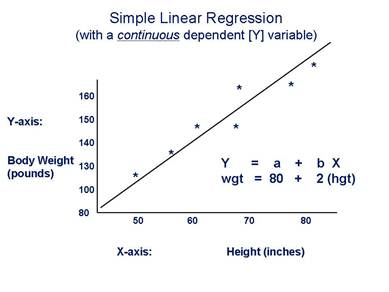
\includegraphics[center]{simpleLinearRegression}
	\caption[Confusion Matrix]
	{Simple Linear Regression}
	\label{fig:simpleLinearRegression}
\end{figure}

We can see from above the $y$ in this example is weight (wgt) and $b_0 + b_1x$ is $80 + 2*Height(hgt)$. This is a very basic example but demonstrates how this can be leveraged for more complex feature sets. Predicting arrears is a dichotomous problem meaning the outcome of the experiment can only have two possible values. 

\subsection{Logistic Regression} \label{LogReg}
\textit{Logistic Regression} \cite[See:][]{hosmer_applied_2000} within the credit scoring industry is one of the most used algorithms \citep{hand_evaluating_2010}. As seen above in Fig. \ref{fig:simpleLinearRegression} a simple regression model outputs a continuous response, in that example body weight. Credit scoring or predicting arrears is a problem where there can only be two possibly values default or not-default, to simplify this we will reduce this to a binary problem where the outcome will be 1 or 0 \citep{zou_modified_2004}. To transform the output of a regression model from $[-\infty, +\infty]$ to a probability between 0 and 1 a logistic transformation is applied. The logistic function can be used to take any value between $+\infty$ and $-\infty$ and output a value between $0$ and $1$. Fig. \ref{fig:logistic_function} below illustrates what a logistic function looks like.


\begin{figure}[H]
	\includegraphics[width=0.6\textwidth, center]{logistic_function}
	\caption[Standard Logistic Regression]
	{Standard Logistic Regression}
	\label{fig:logistic_function}
\end{figure}

The logistic function is defined in Equation \ref{eq:logitReg} as the following: 

\begin{equation} \label{eq:logitReg}
	\text{Logistic Model}  =  p  =  \frac{1}{1 + e^{-(b_0 + b_1x)}}
\end{equation}

As discussed already linear regression is an unsuitable classifier for making dichotomous predictions as linear regression produces predictions for a range beyond 0 to 1. Logistic regression also produces a curved line that is bounded by values between 0 and 1. Fig. \ref{fig:LogRegVsLineReg}

\begin{figure}[H]
	\includegraphics[width=0.6\textwidth, center]{LogRegVsLineReg}
	\caption{Comparison between Linear and Logistic Regression Models}
	\label{fig:LogRegVsLineReg}
\end{figure}

in \ref{fig:LogRegVsLineReg} the constant, $b_0$ dictates the position of the curve which can be moved left and right depending on its value, $b_1$ will be the slope of the curve. 

The logistic regression model can be extended to include any number of interval and nominal variables which is illustrated in Equation \ref{eq:logitRegExtended}

\begin{equation} \label{eq:logitRegExtended}
	p  =  \frac{1}{1 + e^{-(b_0 + b_1x_1 + b_2x_2 +\cdot\cdot\cdot+ b_px_p )}}
\end{equation}

Logistic Regression can also be used in cases where there are more than two outcome groups. For example it could be used in predicting what stage a customer is in the customer lifecycle e.g. Awareness, Interest/Consideration, Evaluation/Purchase, this is referred to \textit{multinomial logistic regression}


One of the main major attractions of logistic regressions it allows you to use discrete, continuous features or a combination of both \citep{lee_application_2005}.

\subsection{K-Nearest Neighbours} \label{kNN}
The \textit{k-nearest neighbour} or {k-NN} for short, is an algorithm that classifies observations based on the how its nearest neighbours are classified. It can be known as the nearest neighbour but in the majority of cases it is useful to use more than one neighbour \citep{henley_k-nearest-neighbour_1996}. The intuition behind this algorithm is that instances which are close by each other will more likely be classified the same way \citep{cover_nearest_1967}. We can see in Fig. \ref{fig:KNN_Example}\\ %added space for small gap in picture 


\begin{figure}[H]
	\includegraphics[width=0.6\textwidth, center]{KNN_Example}
	\caption{Example k-NN, contrasting results for \textit{k}=3 and \textit{k}=5 }
	\label{fig:KNN_Example}
\end{figure}

that results of the algorithm can vary with the choice of \textit{k}. It should also be noted that when applying this algorithm to binary experiment it is good practice to only choose odd values of \textit{k}, this will eliminate the risk of ties from the decision process \citep{keller_fuzzy_1985} 

While adopting the k-NN algorithm you can choose which method and validate what the best distance measure to decide what are your nearest neighbours. There are some common distance measures for continuous features only, Equation \ref{eq:Minkowski} is the \textit{minkowski distance} is one of the most common, where \textit{p=1} this becomes the Equation \ref{eq:Manhatten} the \textit{manhatten distance} and where \textit{p=2} this becomes the Equation \ref{eq:Euclidean} the \textit{euclidean distance}

\begin{equation} \label{eq:Minkowski}
	\text{Minkowski Distance}   = \Big(\sum_{i=1}^k (\abs{x_i-y_i})^p\Big)^\frac{1}{p}
\end{equation}

\begin{equation} \label{eq:Manhatten}
	\text{Manhatten Distance}   = \sum_{i=1}^k \abs{x_i-y_i}
\end{equation}

\begin{equation} \label{eq:Euclidean}
	\text{Euclidean Distance}   = \sqrt{\sum_{i=1}^k (x_i-y_i)^2}
\end{equation}

The results from k-NN will vary depending on your choice of distance measurement, but there more distance metrics for continuous features such as \textit{Correlation Similarity}, \textit{Cosine Similarity} \citep{sarwar_item-based_2001}

Analysis can be completed to evaluate what the optimal value for \textit{k} is based on inspecting the results and creating benchmarks. Anecdotally the larger the value of \textit{k} the more precise the algorithm can be but as with most things in machine learning there are no guarantees. You can leverage methods such as cross validation discussed in Section \ref{subsec:k_fold} and utilised in Chapter \ref{Chapter4} to evaluate what the good choice of \textit{k} would be. It is also a widely used method in synthetic sampling with will be discussed later in the chapter, in Chapter \ref{Chapter4} and Chapter \ref{Chapter5}.

\subsection{Decision Trees} \label{decTrees}
The \textit{decision tree} algorithm classifies observations into classes in the form of tree like structure, hence the name. The algorithm seeks to partition the dataset into smaller subsets, using the relationship between the feature set and target variable to do so. Fig. \ref{fig:decisionTree}

\begin{figure}[H]
	\includegraphics[width=1\textwidth, center]{decisionTree}
	\caption{Simple Decision Tree for Yes, No Prediction \\ \cite[Source:][]{quinlan_induction_1986}}
	\label{fig:decisionTree}
\end{figure}

The output of the algorithm splits the data into smaller subsets of data, which output is a tree with root, internal and leaf nodes. As can be seen in Fig. \ref{fig:decisionTreeExplained}, the root node in this example \textit{Outlook} is the first node in the tree which means it is the most predictive feature. 

\begin{figure}[H]
	\includegraphics[width=.6\textwidth, center]{decisionTreeExplained}
	\caption{Decision Tree with Nodes and Leafs labelled}
	\label{fig:decisionTreeExplained}
\end{figure}

The \textit{root node} will have have two or more branches in this case three \textit{Rainy, Overcast} and \textit{Sunny}. Below these branches you have \textit{internal or split node} \textit{Windy} or \textit{Humidity} which output more branches. The bottom nodes of each decision or branch is the prediction or classification, this is called the \textit{leaf node}. In this example the leaf node decision will be whether or not it will rain represented by Yes/No in Fig. \ref{fig:decisionTreeExplained}

The algorithm that builds decision trees is called the \textit{iterative dichotomiser 3} more commonly known as ID3 by \cite{quinlan_induction_1986}. The algorithm applies a top down approach to choosing its root and internal nodes. The algorithm only evaluates one step ahead from where it is in the decision process at any time and does not allow for any backtracking. This decision making process is known as a greedy approach as it just makes the optimal solution at that stage of the process. Thus because of these limitations the optimal solution is not guaranteed taking this approach \citep{friedman_lazy_1996}.

The ID3 algorithm works by calculating the \textit{entropy} and \textit{information gain} at each step or decision node, where you use the feature with the smallest entropy or feature that maximises information gain.

Entropy $H(S)$ seen in Equation \ref{eq:entropy} measures how much uncertainty there is in the data \citep{shannon_mathematical_2001}

\begin{equation} \label{eq:entropy}
	H(S) = - \sum_{x \in X} p(x) \log_{2} p(x)
\end{equation}
Where:
\begin{itemize}[label=]
	\item $S$: The current dataset entropy is being calculated for, this will change each time entropy is being calculated
	\item $X$: The set of classes in $S$
	\item $p(x)$: Proportion of observation in class $x$ compared to total number in set $S$
\end{itemize}
If $H(S) = 0$ then the observations in $S$ are all of the same class. Entropy is calculated for each feature, the feature with the smallest entropy is used to split at that step.

Information gain is used to measure the decrease in entropy after the dataset is split on a feature. The equation for the information is 

\begin{equation} \label{eq:infoGain}
	IG = H(S) -  H(T)
\end{equation}
Where:
\begin{itemize}[label=]
	\item $H(S)$ is the the entropy of S
	\item $H(T)$ is the entropy of subset T based on splitting data on some feature
\end{itemize}

Information gain is calculated and the feature with the highest gain is chosen to split the dataset. The algorithm then runs recursively until all the data is classified and predictions have been made. 

Multiple decision trees may output the same results. This can be seen in Fig. \ref{fig:simpleComplex} where two different decision trees classify the dataset correctly. \cite{quinlan_induction_1986} suggests that that in scenarios like this the simpler decision tree would be chosen Fig. \ref{fig:simple}

\begin{figure}[H]
	\centering
	\begin{subfigure}[b]{0.45\textwidth}
		\captionsetup{font=scriptsize}
		\includegraphics[width=\textwidth, height=5cm]{decisionTreeSimple}
		\caption{Simple Decision Tree}\label{fig:decisionTreeSimple}
		\label{fig:simple}
	\end{subfigure} ~\quad
	\begin{subfigure}[b]{0.45\textwidth}
		\captionsetup{font=scriptsize}
		\includegraphics[width=\textwidth,height=5cm]{decisionTreeComplex}
		\caption{Complex Decision Tree}\label{fig:decisionTreeComplex}
		\label{fig:complex}
	\end{subfigure}
	\caption{Simple and Complex Decision Tree Comparison\\\cite[Source:][]{quinlan_induction_1986}}
	\label{fig:simpleComplex}
\end{figure}

This is done because the simpler the rules of the tree the more likely the tree is to generalise well on unseen data. In other words if the tree is too complex it is more than likely over-fitting the training dataset. There is also a computational cost to classifying complex trees. 

There are also other issues to be aware of when building a classifier using a decision tree. Information gain can be biased to features that have a large number of values. These features will result in a root node that produces a very broad or wide tree that classifies the training data well or perfectly but performs very poorly in unseen cases. One scenario where this could happen would be if you used the unique identifier of each record in as a training input, this model would perform very well in training but would not perform well on unseen data. There are methods to mitigate the the risk of over-fitting against these features \textit{gain ratio}, \textit{symmetric uncertainty} and the \textit{gini index}. \cite{quinlan_induction_1986} noted that using these methods for node decision often found favourable results compared with information gain. It should be noted also that these metrics can be using in the feature selection process where not related to building decision trees


\subsection{Artificial Neural Networks} \label{neuralNets}
The \textit{artificial neural network} (ANN) is learning algorithm that is based on an understanding of how neural networks, such as our brain learns. Motivation to study how ANN comes from the success of how the human brain was faster than the worlds fastest computers at certain applications such as object recognition, speech recognition and general perception \citep{haykin_neural_1998}.

As a human grows their brain develops, learns and creates a set rules based on the experiences it has had. These rules and experiences are stored in approximately 100 billion neurons or nerve cell in the brain. These neurons are connected in a network and use this as a method of communication sending electrical and chemical signals back and forth between neurons. On their own each neuron is not very useful but combined and with communication has allowed humans to learn and grow so successfully. 

An ANN seeks to replicate the neural network of the human brain, albeit on a much smaller scale. It does this by taking advantage of powerful computers which carry out a lot of simple tasks very quickly. ANN have proven their value from their ability to map out any non-linear function \citep{white_learning_1989} and their prowess in applications such as pattern and speech recognition and forecasting \citep{kaastra_forecasting_1995}.

Fig. \ref{fig:annFotwardFeeding} shows a common layout of an ANN. Like in the brain the ANN is comprised of processing neurons usually known as nodes which are organised into three layers, input, hidden and output. Between layers nodes are connected and as seen in Fig. \ref{fig:annFotwardFeeding} each connection may carry a different weight.

\begin{figure}[H]
	\includegraphics[width=.6\textwidth, center]{annFotwardFeeding}
	\caption{Three-layered feed-forward artificial neural network configuration \\
				\cite[Source:][]{raju_development_2011}
			}
	\label{fig:annFotwardFeeding}
\end{figure}

Data comes in through the input layers nodes and is fed through the network, from the input to the hidden and then onto the output layer. In the hidden layer each node calculates a sum based on the input node and the weight of the connection, these hidden nodes then pass on values to the nodes in the outer layer where another calculation which converts the value to a value between 0 and 1 by passing it through the sigmoid function seen in Fig. \ref{fig:logistic_function}. Throughout the training process the connection weights are changed and tested against in order for the ANN to learn and improve its predictions \citep{haykin_neural_1998}

Although ANN have become increasingly popular in recent years due to improvements in the algorithms, the the increase in computer power and success in application such as object and speech recognition,  some are still sceptical because of the "black box" nature of their results, where users do not know what the internal workings of the algorithm are  \citep{kaastra_forecasting_1995}. 



\subsection{Support Vector Machines} \label{SVM}
A Support Vector Machines (SVMs) learning was developed first by \cite{vapnik_nature_1995}. The algorithm performs classifications via a hyperplane in a higher dimensional feature space that maximises the margin or distance separating the two classes. It can be seen in Fig. \ref{fig:svmExample} that the two class are linearly separable using the hyperplane in the higher dimensional feature space. 

\begin{figure}[H]
	\includegraphics[width=.5\textwidth, center]{svmExample}
	\caption{Optimal separating hyperplane in SVMs of feature space \\
		\cite[Source:][]{li_adaptive_2011}
	}
	\label{fig:svmExample}
\end{figure}

SVM handles situations non-linear data by using kernel function (non linear) to transform the data into a higher dimensional feature space. This allows it to become linearly separable via a hyperplane, this is known as the \textit{kernel trick}. It can illustrated in Fig. \ref{fig:svm_nonLinearlySeperable} by transforming non linearly seperable data into a higher dimensional feature space where it can be linearly separated using a hyperplane. This is ability is what differentiates SVM from logistic regression.

\begin{figure}[H]
	\includegraphics[width=.5\textwidth, center]{svm_nonLinearlySeperable}
	\caption{SVM classifying non-linearly classes \\
		\cite[Source:][]{burges_tutorial_1998}
	}
	\label{fig:svm_nonLinearlySeperable}
\end{figure}

It has been documented across a range of domains where SVMs are performing well such as credit risk evaluation \cite{van_gestel_credit_2009} and text categorisation, cancer diagnosis and pattern recognition \citep{shin_application_2005}

\subsection{Ensemble Models \& Boosting} \label{boosting}

In 1907, mathematician Sir Francis Galton went a market in which there was a challenge
to approximate the weight of an Ox. After evaluation the 787 forecasts made by the
participants, he noticed that while there was a large variance in the guesstimate
with large deviations from the correct weight, the median value of the
forecasts was less than 1\% away from the correct weight of the Ox \citep{galton_vox_1907}. Although the failings of the separate guesses, the united wisdom of the every guess generated a very accurate estimate. This is a similar how ensemble models are generated.


Boosting relates to an powerful principal of generating a very accurate prediction model using an aggregation of reasonably inaccurate ``rules of thumb'' \citep{freund_short_1999}. A frequently utilised ensemble is the Adaptive Boosting algorithm which frequently called AdaBoost in the literature. A weak learner is produced from the first iteration where all observations are are potentially to be chosen. For later sampling of the distribution the model adjustments are made bases on the error rates of the classifier so that model will look at samples of data were incorrectly classified \citep{freund_short_1999}. This way the algorithm is step by step adapting based on the errors of past classifications and then focuses correcting the record labels it got incorrect. A specific method of AdaBoost is the Boosted-Stumps Model. This is an ensemble model that leverages decision tree stumps, these are decision trees with one split. This method is seen to be optimal to common AdaBoost which tends to over-fit the training dataset \citep{caruana_empirical_2006}.

Bagging is an alternative method employed to generate ensemble models levering decision trees. One method of bagging is \textit{bootstrap replica}. This method works on the principal for a dataset of size $n$ that will be used to train a model, it generates trees using just different partitions of the training data with replacement \citep{dietterich_experimental_2000}. Random forests are another example of an ensemble model generated using multiple decision trees. A large number of decisions trees will be trained and results are combined together to make a classification, hence why its called a forest. Each decision tree is trained on random subsets of the features available hence why its called a random forest. Research provided by \cite{breiman_random_2001} demonstrated that the random forests performed better on tests compared to AdaBoost method across a variety of datasets.


\section{Feature Selection}\label{sec2:featureSection}
Feature selection is a process of choosing the best subset of features from the full dataset for you scoring model by excluding features that have been to be redundant. \cite{guyon_introduction_2003} discusses that feature selection methods are usually split into one of three categories (i) filter techniques (ii) wrapper techniques (iii) embedded techniques. 

\subsubsection{Filter Methods}
Filter feature selection methods use statistics to to assign a score for each feature versus the target. The features are then ordered by which are most predictive and a decision is made what ones to keep. Filter method techniques include information gain, correlation coefficient and the chi squared test.

\subsubsection{Wrapper Methods}
Wrapper feature selection method evaluates various subsets of features together while scoring the model for each subset. The different model results are then evaluate and compared against the other results returning the result which returned the best based on the model evaluation criteria. Forward, backward and general stepwise regression are very common techniques of wrapper methods being used.

\subsubsection{Embedded Methods}
Embedded feature selection method attempts to combine the two previous methods together. That is, the method looks to learn what features are useful as the model is being created. 

Feature selection is very important in the credit scoring process and there are many reasons in the literature that suggest it should be used. The \textit{curse of dimensionality} is one such issue, if you have too many features in your model it may perform well on the training dataset but when executed on unseen data it may perform poorly because the model has over-fitted too many irrelevant or noisy features \citep{loughrey_overfitting_2005}.Research from (\cite{thomas_consumer_2009}; \cite{mays_credit_2004})  advise that to build a robust scoring model you should have somewhere between 8 and 20 predictive features. There are many reason for this, there is a practical issue having to model more features and there are costs and overheads associated with each features that is redundant in the model. Referencing Fig. \ref{fig:simpleComplex} we can see that is much desirable to have simple decision tree than a complex decision tree with the same outputs, likewise if two datasets are providing the same results only one is a subset it is always better to choose the subset. This way we will reduce the risk of over-fitting that goes with including redundant features.

\section{Coarse Classification} \label{sec:binning}
Coarse classification is often utilized to transform the predictive features into a simpler form which is better suited for modelling \citep{carroll_transformation_1988}. Coarse classification is also referred to in the literature as binning, grouping, discretisation. For continuous and categorical feature values are transformed into a small number of bins or groups. These values  are mapped into these groups by referring to the target feature to identify the optimal cut-off points. 

Coarse classification has many benefits one is that it allows one you to capture some of the features non liner relationship with the target feature. This is done each category in the group being treated as its own dummy variable which will have its own weight in a logistic regression model \citep{hand_optimal_2005}. Coarse selection can also increase the overall robustness of the model by reducing the possibility of over-fitting by creating groups with the optimal number of good and records \citep{baesens_50_2009}. It also gives you the capability of mitigating against the risk or outliers and missing values. 

Coarse classification is also very quick to deploy, previously it would have been completed by analysts iteratively complete the process which was a very time consuming process. Algorithms now such as chimerge and recursive partitioning to name a few, find optimal cut-points in the features quickly and accurately. Those groups are then evaluated using the \textit{Weight of Evidence} (WoE) and \textit{Information Value} (IV) \citep{garcia_survey_2013}. 

A common methodology to coarse classification is to break up each feature into roughly three to six bins or groups \citep{hand_optimal_2005}. It is recommended that bins are limited to six to ensure the model does not become over-parameterised and difficult to manage. Contrarily, the model will become too rigid less than three groups are used. 

Approximating the WoE of each bin, and tuning where optimal is the most known method to carrying out coarse selection \citep{thomas_consumer_2009}. In a credit scoring problem the WoE for bin $i$ is defined as 
  
\begin{equation} \label{eq:woe}
\text{WoE} =  \ln\bigg(\frac{n_g(i)}{n_b(i)} \bigg/ \frac{N_g}{N_b}\bigg)
\end{equation}

where the amount of goods in a bin $i$ is $n_g(i)$, and the amount of bads in a bin $i$ is $n_b(i)$. $N_g$ and $N_b$ are the total amount of goods and bads in the full dataset. A negative WoE signals that a bin is more likely to default, whereas a positive WoE signals they likely to not default.

The information value is frequently applied frequently with the WoE. The IV is powerful method ranking variables by their importance which can be used for feature selection in the prediction model. The IV suggests the predictive capability of a binned feature, it is defined as  
 
\begin{equation} \label{eq:informatoValue}
\text{IV} =  \sum\limits_{i=1}^j \bigg(\frac{n_g(i)}{N_g} -   \frac{n_b(i)}{N_b}\bigg) * \text{WoE$_i$}
\end{equation}

where $j$ is the amount of bins in a feature. The IV of each bin is known as a contribution, which are then added together to generate the IV of a feature.

In general binned features with an IV between 0.3 and and less than 0.5 are thought to be very predictive features \citep{mays_credit_2004}. If the the IV is more than 0.5 it could be over-fitted or it could be a anachronistic feature and should be examined further \citep{si} \citep{siddiqi_credit_2012}. Binned features with an IV of smaller than 0.1 is thought to be weaker features and could be considered to be removed from the model \citep{anderson_credit_2007}.

\begin{comment}
\subsection{Correlation-based Feature Selection}
\subsection{Information Gain}
\subsection{Coarse Classification/ Binning}
\end{comment}

\section{Class Imbalance Problem}\label{sec:imBalance}
One of the biggest assumptions that needs to be understood when using classification algorithms is that most assume there is a balanced distribution of the target class \citep{japkowicz_class_2000}. Target class imbalance is described by  \citep{chawla_smote:_2002} where the number of number of records in each class are not relatively equal. In a balanced dataset ratio between the a binary target class would be close to 50/50. The issue with this imbalance arises where algorithms assume there is a balance between the classes, and they attempt to maximise the accuracy by predicting the most common class \citep{drummond_severe_2005}. The algorithms attempt to minimise the classification errors, but do not accounts for the incorrectly classifying cases \citep{seiffert_improving_2009}. While these classification overall might be very accurate they are not very useful in real world problems, this is because in the majority of cases the algorithm will focus on the majority class, because of how heavily it is weighted in the training dataset ignoring the minority class. This is major problem because in the majority of cases you will trying to predict the minority class, in this thesis customers going into default is the minority e.g. there are more customers that do not default at the end of the outcome window than customers that do defaulters.

The study of class imbalance has started to receive more and more attention in relation to data mining and machine learning in recent times. \cite{weiss_mining_2004} discusses what the role and issue that rare class instances can play in data mining. \cite{weiss_mining_2004} makes the distinction that there are two types of class imbalance which depend on the type of rarity in the data, these are called \textit{absolute rarity} and \textit{relative rarity} which are discussed next.

The major issue with rarity is there is a simply a lack of data in real world problems. Absolute rarity occurs when the number of instances related to the rare class is very small in an absolute sense. Lack of data means it is difficult to identify what leads to a rare class. Fig. \ref{fig:absoluteRarity} illustrates how absolute rarity can become an issue.

\begin{figure}[H]
	\includegraphics[width=0.6\textwidth,center]{absoluteRarity}
	\caption{
		Impact of Absolute Rarity in Data Mining \\ \cite[Source:][]{weiss_mining_2004}
	}
	\label{fig:absoluteRarity}
\end{figure}

It can be seen on the left side of Fig. \ref{fig:absoluteRarity} that there is only one rare/positive example, compared to the right where there is more data this more rare cases. It can be observed that the decision boundary on the right side for when there is more data is much more accurate than on the left side when there is just one observed rare class. This is a simple illustration that having more data should allow you to make better predictions. Relative rarity is where classes are not rare in an absolute sense but are rare relative to other objects. A supermarket example can illustrate this better, imagine you want to identify the relationship between two items, but these items are rarely purchased as whole, so even if they happen to be purchased together the relationship may be difficult to identify.

As mentioned previously, very often in the real world problems imbalance exists in the dataset, thus there has been researched completed that have identified methods of mitigating against this risk. \citep{chawla_editorial:_2004} proposes solutions fine tuning the algorithm and manipulating the data. 

\subsubsection{Manipulating the data} \label{sec:dataManip}

A method of manipulating the data is to resample to data with the aim of balancing the distribution of the target class. Solutions proposed,

\begin{itemize}
	\item Random undersampling of the majority class
	\item Random oversampling of the minority Class
	\item Synthetic sampling of the minority Class 
\end{itemize}

A very common method used is to randomly oversample the minority class in your training set, one of the biggest issues with this is that you are increasing your chances of over-fitting the algorithm the training model as it been training on multiple copies of the same data which are not adding any new information. However over-fitting can be issue with this approach as the algorithm becomes biased and skewed on the training data, thus ends up performing poorly on the validation and test data \cite[see][]{hawkins_problem_2004}

Random undersampling of the minority class is where random samples of the training dataset that are part of the majority class are removed. This means number of minority classes remains unchanged but the majority class is reduced, thus the overall class balance becomes more even. The issue that arises from undersampling is that there is possibility that you removes the important information from the training dataset that is used for predicting that class. It should be noted \cite{kennedy_credit_2013}, that undersampling the majority class is not a useful solution for the issue of absolute rarity.

Synthetic sampling  is alternative method to randomly oversampling the minority class. New data items are added to the training set but unlike oversampling which adds duplicate records the records added are dummy or made up in a way to look similar and taking characteristics of the already existing records, thus they are not duplicates but synthetic. One method for creating synthetic data was proposed by \citep{chawla_smote:_2002} where data was generated by creating data items using K-NN where the item would sit between minority classes.

\begin{figure}[H]
	\centering
	\begin{subfigure}[b]{0.32\textwidth}
		\captionsetup{font=scriptsize}
		\includegraphics[width=\textwidth]{SMOTE_Before}\caption{}
		\label{fig:SMOTE_Before}
	\end{subfigure}  ~\quad
	\begin{subfigure}[b]{0.32\textwidth}
		\captionsetup{font=scriptsize}
		\includegraphics[width=\textwidth]{SMOTE_After}
		\caption{}
		\label{fig:SMOTE_After}
	\end{subfigure}
	\caption{Fig. \ref{fig:SMOTE_Before}: Example of the K-NN for $x_i$ using $k = 6$. \ref{fig:SMOTE_After}: Data created using SMOTE based on the euclidean distance.\\
		\cite[Source:][]{he_learning_2009}}
	\label{fig:smoteExample}
\end{figure}

Above in Fig. \ref{fig:smoteExample} it is illustrated how synthetic data using the SMOTE methodology can be generated. For the purposes of this thesis this will not be discussed further.

\subsubsection{Fine tuning the algorithm}
There are ways to also cater for the target class imbalance of the dataset by fine tuning the algorithm. One method which is illustrated in Chapter \ref{Chapter4} of this thesis is to adjust the cut-off or threshold parameter value for the model, \cite{provost_machine_2000} warns that it would \textit{``critical mistake"}. In Section \ref{modelPerformMeasure} model performance measures, it is  worth noting that \cite{chawla_editorial:_2004} suggests using evaluation measures such as accuracy which rely on a specific threshold could lead to misleading results when the target class is imbalanced, they instead recommend using ROC and AUC to get a more accurate predictions, this similar to industry standards in terms of handling the imbalance.

This section has detailed some of the concern that imbalance can cause when building predictive models, we have outlined some the solutions and methods to mitigate this by manipulating the data and fine tuning the classification algorithm.


%----------------------------------------------------------------------------------------
%	SECTION 7
%----------------------------------------------------------------------------------------
\section{Model Validation Methods}\label{sec:modelValid}
In machine learning historic data is used to build a model to make future predictions based on past information. Classification algorithms like the ones already discussed in this section need to validated and tested. This section details some methods and approaches to tackling this problem so the predictions from the model are useful which has been discussed extensively in \citep{refaeilzadeh_cross-validation_2009}

\subsubsection{Holdout Validation}
The \textit{holdout validation} method is used to avoid the over-fitting issue discussed in the resubstitution method. The idea is to split the data into partitions, one for training and one for testing. The algorithm is only trained on the test data, this allows for the model to generalise much better on unseen data, overall producing a much better prediction model. This method has an issue however where one, not all the data is used for training, and two the results can be dependent on the how and what data are used for training and testing. Examples where this could become an issue is important information in the data for training is lost in the test partition, or the instances chosen for test may be too easy or too difficult to classify, this may cause your results to be skewed and making your predictions bias to that testing partition. 

The hold-out method can also incorporate a third subset called the \textit{validation set}. In the case the dataset is partitioned into three partitions train, validation, and test. The validation sets purpose is to fine tune models parameters, for example selecting the best threshold cut-off measure for a model or performance measure. It is not required always for building predictive models. 

\begin{figure}[H]
	\includegraphics[width=0.6\textwidth,center]{holdout}
	\caption{Example of Holdout Data Split with Training and Test Data}
	\label{fig:holdout}
\end{figure}

Fig. \ref{fig:holdout} illustrates how the complete dataset is partitioned into a training and test sets. 




To address the biasses is Holdout you could re-run multiple tests and average the results, or more commonly you could look at using \textit{k-fold cross-validation} discussed in the next subsection.

\subsubsection{K-Fold Cross Validation}\label{subsec:k_fold}
The \textit{k-fold cross validation} can be used to deal with the bias issues discussed above. The first step of this method is to split the data into $k$ equally sized partitions called folds. A model is then trained using $k$ iterations, where for each iteration a different fold of data is used for testing and training the model. This can be illustrated well below in Fig. \ref{fig:5-fold-cv} where there are 5-folds, and for each iteration you can see different fold is being used for testing.  

\begin{figure}[H]
	\includegraphics[width=0.7\textwidth,center]{5-fold-cv}
	\caption{5-Fold Cross Validation}
	\label{fig:5-fold-cv}
\end{figure}

It is important and usually common practice that each fold is representative of the the whole dataset, for each example that the target class ratio split is the same for each fold as for the entire dataset. 

\subsubsection{Leave-One-Out Cross-Validation}
The \textit{leave-one-out cross-validation} (LOOCV) method is a specialised version of $k$-fold cross-validation, where $k$ is equal to the number of observations in the dataset. In layman's term this means all the data bar one observation is utilized training the model, and testing is done on one observation. This is completed for each observation in the dataset. Although it is worth noting that accuracy estimate gathered using this method produces unbiased results, it also high variance which can lead to misleading results \citep{refaeilzadeh_cross-validation_2009}.
 

\subsubsection{Repeated K-Fold Cross Validation}
The \textit{repeated k-fold cross validation} method is another specialised version of $k$-fold cross-validation. In an attempt to improve the performance of the model using this method $k$-fold cross-validation is rerun multiples times. Each time it is rerun the data is shuffled so data will appear in different folds for each repeat run. 

\subsubsection{Summary}

Holdout and cross validation methods are both used extensively for evaluating how measuring the performance of the models. In the majority of cases if there is a large enough dataset you might choose to just use holdout method, but in some situations of you may want to use cross validation.

There are considerations that need to be thought about before using either, hold-out is simple can be implemented easily and quickly and can be rerun multiple times to get a more unbiased result. K-fold is again theoretically simple but may not be a simple to implement as the code may be tedious and time consuming where the gains may not be worth the investment in industry. 

\citep{kohavi_study_1995} and \citep{salzberg_comparing_1997} both performed research on approaches to choosing the correct validation method. \cite{kohavi_study_1995} analysed many cross validation methods, regular, leave-one-out, stratified. They came to the conclusion that 10-fold cross-validation produced the most accurate and unbiased results. \cite{salzberg_comparing_1997} also studies the issues of comparing model performance and proposes a solution that combines k-fold cross validation combined appropriate hypothesis tests opposed to evaluating the average accuracy.   



%----------------------------------------------------------------------------------------
%	SECTION 8
%----------------------------------------------------------------------------------------
\section{Model Performance Measures}\label{modelPerformMeasure}

This section details some of the metrics that can be used to assess the accuracy of a classifier. The result of the classification algorithm maps the modelled data into a category, in this thesis it a binary classifier that is output: 1 is output for identifying customers who will default (bad) or 0 is output for customers who will be not-default (good). The majority of classification algorithms will produce a ranked numeric value which can be converted to a binary representation by some threshold or cut-off decision driven from  the business objective that is trying to be optimised. This section will begin with a confusion matrix, details how this is leveraged to build other performance measures and details how charts and metrics can be leveraged together to decide on the performance measure to maximise the intended objective.

\subsubsection{Confusion Matrix}

The results that made by the classification algorithm can be represented by a contingency table known as a confusion matrix. In this thesis the classification algorithm will output a binary classification, so the confusion matrix will be made from a $2 \times 2$ matrix that has two classes, known as the \textit{positive} and \textit{negative} class. For this thesis, the positive class will be the customers that default and negative class will be the customers that do not default. It will illustrate what proportion of correct and incorrect predictions were made with respect to the target.The confusion matrix can be broken down into the following categories for this thesis:

\begin{itemize}
	\item \textit{true positive} (TP), cases that are predicted to default, and are {\color{green}{correctly}} classified as \textit{positive}
	\item \textit{false positive} (FP), cases that are predicted to default, and are {\color{red}{incorrectly}} classified as \textit{positive}, also known as \textit{Type I error}.
	\item \textit{false negative} (FN), cases that are predicted to not-default, and are {\color{red}{incorrectly}} classified as \textit{negative}, also known as \textit{Type II error}.
	\item  \textit{true negative} (TN), cases that are predicted to not default, and are {\color{green}{correctly}} classified \textit{negative}
	
\end{itemize}

Fig \ref{fig:ConfusionMatrix} illustrates how information from a confusion matrix can be presented and read.

\begin{figure}[H]
	\includegraphics[width=0.8\textwidth,center]{Confusion_Matrix}
	\caption[Confusion Matrix]
	{Confusion Matrix}
	\label{fig:ConfusionMatrix}
\end{figure}

Using the numbers outputted from the confusion matrix, model evaluation measures can calculated and evaluated for the required objective, measures such as \textit{accuracy} (Equation \ref{eq:Accuracy}) which measures proportion of the number of predictions that were correct, the \textit{misclassification rate} (Equation \ref{eq:Misclassification Rate}) what proportion of predictions were wrong, the \textit{sensitivity} (Equation \ref{eq:Sensitivity}), otherwise known as \textit{recall} or the \textit{true positive rate} (TPR), measures the proportion of the positive instances that are correctly identified i.e. proportion default cases that have been predicted correctly. \textit{Specificity} (Equation \ref{eq:Specificity}) measures the proportion of negative cases that are predicted correctly i.e. proportion of non-default cases that have been predicted correctly, \textit{precision} (Equation \ref{eq:precision}) measures when the classifier predict positive outcomes what proportion are correct, \textit{negative predictive value} (NPV) (Equation \ref{eq:npv}) measures the proportion of negative predictions that were correct i.e. if the classifier predicted the outcome would be non-default what proportion were correct. One measure that can be very useful when the where there is class imbalance is \textit{balanced accuracy} (Equation \ref{eq:Balanaced Accuracy}), \citep{brodersen_balanced_2010} discusses how using this negates the impact of bias or skewness from the more frequent class

\begin{equation} \label{eq:Sensitivity}
\text{Sensitivity} = \text{Recall} = \frac{TP}{TP + FN}
\end{equation}

\begin{equation} \label{eq:Specificity}
\text{Specificity} = \frac{TN}{FP + TN}
\end{equation}

\begin{equation} \label{eq:precision}
\text{Precision} = \frac{TP}{TP + FP}
\end{equation}

\begin{equation} \label{eq:npv}
\text{Negative Predictive Value} = \frac{TN}{TN + FN}
\end{equation}

\begin{equation} \label{eq:Accuracy}
\text{Accuracy} = \frac{TP + TN}{TP + FP + FN + TN}
\end{equation}

\begin{equation} \label{eq:Balanaced Accuracy}
\text{Average Accuracy} = \text{Balanaced Accuracy} = \frac{Sensitivity + Specificity}{2}
\end{equation}

\begin{equation} \label{eq:Misclassification Rate}
\text{Misclassification Rate} =  \frac{FP + FN}{TP + FP + FN + TN} = 1 - \text{Accuracy}
\end{equation}

\begin{figure}[H]
	\includegraphics[width=0.8\textwidth,center]{Confusion_Matrix_Example}
	\caption[Confusion Matrix Example]
	{Confusion Matrix Example}
	\label{fig:ConfusionMatrixExample}
\end{figure}

Fig. \ref{fig:ConfusionMatrixExample} illustrates how the TP, FP, FN, TN can be used to create performance metrics for classification algorithm. As discussed already confusion matrix based performance measures are built on the threshold that is selected for converting the predicted numeric score into a binary outcome. Anecdotally you might believe that the cut-off or threshold of 0.50 is acceptable but this rule may not always especially if there is an imbalance between the positive and negative class in the dataset. The cut-off should should ideally be based on you business objective where you look to minimise, maximise and analyse the trade off as you alter the cut-off. 

The confusion matrix is not the only way to evaluate the performance of the classification algorithm and is not always advocated in the literature or by industry. In studies completed by \citep{lessmann_benchmarking_2008} choose not to select a classification cut-off arguing that studies comparing the same dataset and classifier could come to the different conclusions.

As mentioned in this section the confusion matrix measures the performance of classifier at a specific threshold, this can be leveraged to create graphical representations of the overall fitness of the model at any threshold. One such method that will be discussed in the next section is the \textit{receiver operating characteristic} (ROC). 


Confusion Matrix is used to evaluating a model where you have divided the output into distinct or discrete categories. A confusion matrix can be reconstructed for any point on the ROC curve. ROC is also is directly related to two other performance methods \textit{area under the curve} and \textit{gini} which will also be discussed.  

\subsubsection{ROC Chart, AUC and Gini Coefficient}
%\url{https://staesthetic.wordpress.com/2014/04/14/gini-roc-auc-and-accuracy/}
The ROC chart is used to evaluate and illustrate how well the evaluate the model fit, this can be a quick test to see if the model generalises well from the test data, to validation and test data. Fig. \ref{fig:ROC} illustrates on the \textit{x-axis} the false positive rate, and on the \textit{y-axis} the true positive rate is represented. As mentioned previously the points on the ROC chart are generated from confusion matrix built from many cut-off or threshold value between $\theta \in [0,1]$. Fig. \ref{fig:ROC} conceptually illustrates how the ROC chart is generated for varying thresholds. 

\begin{figure}[H]
	\includegraphics[width=0.8\textwidth,center]{ROC}
	\caption[ROC]
	{ROC Chart Example with thresholds 0.65 \& 0.50}
	\label{fig:ROC}
\end{figure}

Fig. \ref{fig:ROC} also illustrate how point (0,1) represents \textit{perfect classification}, that is the classifier correctly predicts all outcomes. 

The ROC chart is basically a combination of confusion matrices over many cut-off values of a classifier. As you can see above finite number of observations in the dataset dictates the number of thresholds that can be used to generate a ROC chart.

To compare ROC chart results of different classifiers the \textit{area under the ROC curve} (AUC) \citep{bradley_use_1997} \& \citep{hanley_meaning_1982}. In Fig. \ref{fig:ROC} the area under the blue ROC line represents the AUC, which is intuitively the area under the curve. In the case of perfect classification this value will be 1, for a random classifier the AUC would be 0.5. 

It is worth noting that AUC does not give total probability of the classifier, and also its usefulness when combined with the ROC to evaluate your classifier across training, validation and test datasets. For example if the ROC curve shifts significantly or is not similar from training to validation/test it suggests that there is possible over-fitting and the model does not generalise well. Also it is worth looking out for a drastic change in the AUC from training to validation/test another sign the classifier does not generalise well may not be useful for predictions. Because of this it is a very strong measure for classifier selection, ROC don't tend to cross over, therefore when comparing two classifiers the one which AUC is higher will be the better classifier independent of the threshold or cut-off.

It is illustrated in Fig. \ref{fig:matric_compare} how the performance measures for confusion matrices vary for different thresholds, but again to keep in mind that it there be just one measure for the AUC of the this ROC Chart.   

\begin{figure}[H]
	\centering
	\begin{subfigure}[b]{0.45\textwidth}
		\captionsetup{font=scriptsize}
		\includegraphics[width=\textwidth]{Confusion_Matrix_threshold_065}
		\caption{Threshold $=.65$}\label{fig:Threshold65}
	\end{subfigure} ~\quad
	\begin{subfigure}[b]{0.45\textwidth}
		\captionsetup{font=scriptsize}
		\includegraphics[width=\textwidth,height=2.025cm]{Confusion_Matrix_threshold_050}
		\caption{Threshold $=.50$}\label{fig:Threshold50}
	\end{subfigure}
	\caption{Confusion Matrix: Multiple Threshold Comparison}
	\label{fig:matric_compare}
\end{figure}

A metric that is commonly used for in \subjectname, industry credit scoring is the \textit{gini coefficient} this is discussed in \citep{hand_good_2005}, this is equates to twice the area in between the diagonal of a random classifier and the ROC curve. The equation for this can be seen below in Equation \ref{eq:gini}

\begin{equation} \label{eq:gini}
\text{Gini} = 2*\text{AUC} - 1
\end{equation}

Just like using a threshold there are limitations to using the AUC and Gini to measure classifier performance, although extremely useful for analysing the performance of wide range of thresholds but not as useful when trying to maximise the performance over a narrow range of thresholds. It cannot tell us the optimal threshold for classifier for  other statistical needs.

One statistic that is commonly used in credit scoring in \subjectname\, industry and in the literature is the \textit{kolmogorov-smirnov} (KS) statistic, this will be discussed in the next subsection.
	

\subsubsection{K-S Chart}\label{subsub:ks}
%\url{http://www.saedsayad.com/model_evaluation_c.htm}
The KS chart and more specifically the KS statistic is one value between 0 and 1. It can be used by measuring the performance of the classifier, by measuring the maximum distance between the cumulative positive and negative distributions of the predicted positive and negative class \citep{seliya_study_2009}. In other words K-S is a measure that illustrates the maximum separation between the positive and negative distributions, this can illustrated more clearly in Fig. \ref{fig:ks}. Another way of thinking KS statistic is that it is point on the ROC curve which is furthest away from diagonal, when measuring perpendicularly. The KS statistic is heavily used in industry as a method for calculating the threshold value for a prediction model \citep{hand_good_2005}. 

Fig. \ref{fig:ks} how the KS statistic and chart is generated, probabilities from the classifier are ordered, grouped and aggregated, but importantly they are separated by the positive and negative class, creating a distribution for each. These two distributions are then plotted separately, you can see in Fig. \ref{fig:ks} that the KS statistic is 47.4\%. This is calculated by taking maximum difference between the two distributions at each group. At group 400-500, if you were to classify all the score are positive below or in this group you would be identifying 81.7\% of the positive instance and only 34.3\% of the negative class, if this was a balanced dataset this could be a very valuable result and measure. 

\begin{figure}[H]
	\includegraphics[width=0.8\textwidth,center]{ks}
	\caption[Kolmogorov-Smirnov chart ]
	{Kolmogorov-Smirnov Table \& Chart }
	\label{fig:ks}
\end{figure}

There are extreme cases of the KS statistic that are worth noting, on is where the KS statistic is equal to 100, this means the scores for each distribution (positive/negative) are but into two separate groups, where one group would just have positive cases and the other just negative case. Alternatively if the model is not very useful and cannot tell the positives from the negatives, it will be like the model is selecting cases randomly and will return a KS statistic of 0.
 

\subsubsection{Gain \& Lift}
The \textit{gain} \& \textit{lift} measure the performance of the classifier. One example where these measure as charts are extremely useful is when communicating in industry with management, they are easy to explain and intuitive where the business can derive and understand value immediately. Fig. \ref{fig:GainLiftWorkflowCharts} below illustrates how the gain and lift charts are generated. 

\begin{figure}[H]
	\centering
	\begin{subfigure}[b]{0.90\textwidth}
		\captionsetup{font=scriptsize}
		\includegraphics[width=\textwidth,height=4cm]{gains_ratio_process}\caption{Process}\label{fig:gains_ratio_process}
	\end{subfigure} 
	\medskip
	\newline
	\begin{subfigure}[b]{0.45\textwidth}
		\captionsetup{font=scriptsize}
		\includegraphics[width=\textwidth]{gains}
		\caption{Gain Chart}\label{fig:gains}
	\end{subfigure} ~\quad
	\begin{subfigure}[b]{0.45\textwidth}
		\captionsetup{font=scriptsize}
		\includegraphics[width=\textwidth]{lift}
		\caption{Lift Chart}\label{fig:lift}
	\end{subfigure}
	\caption{Gain \& Lift Work-flow \& Charts}
	\label{fig:GainLiftWorkflowCharts}
\end{figure}

The charts above illustrate how much likely it is we receive positive responses using the classifier compared to use a random model. The population in the dataset are broken into deciles, which can be seen in \ref{fig:gains} \& \ref{fig:lift}. An example of how they can be used is if we were to evaluate the first 10\% of the population identified by the classifier it would outperform a random selection of customers that would turn out to positive by 3.6.

Essentially these charts are visual aids which can be leveraged for evaluating the performance of the classifier. 

%----------------------------------------------------------------------------------------
%	SECTION 9
%----------------------------------------------------------------------------------------
\section{Conclusion}\label{sotaConc}
This chapter has summarised the relevant literature available for ...
%----------------------------------------------------------------------------------------
%	SECTION 6
%----------------------------------------------------------------------------------------
